\section{\texorpdfstring{Instrukce a strojový kód}{Instrukce a strojovy kod}}

% =====================================================================================================================
	\begin{frame}
    \frametitle{Strojový kód STM8S208RB}
		
		\textbf{Instrukce:}
		\begin{itemize}
			\item jsou dlouhé 1 až 5 bytů a mají různou dobu zpracování,
			\item obsahují informace o operandech,
			\item obsahují informace o způsobu adresování (adresovací režim).
		\end{itemize}
		
		\vspace{3mm}
		\textbf{Strojový kód:}
		
		\begin{itemize}
			\item je obsahem souboru HEX, kde jsou operační kódy instrukcí řazeny za sebou,
			\item neexistuje oddělovač - délka instrukce je zřejmá z jejího operačního kódu,
			\item HEX by bylo možné vytvořit přímo, ale je to extrémně obtížné - používáme jazyk symbolických adres, tj. assembler a překladač,
			\item disassembler - získáme instrukce v assembleru, ale místo názvů proměnných budou adresy.
		\end{itemize}

	\end{frame}
	
% =====================================================================================================================
	\begin{frame}
    \frametitle{Instrukce Load z datového listu STM8S208RB}
		
		
		\begin{center}
			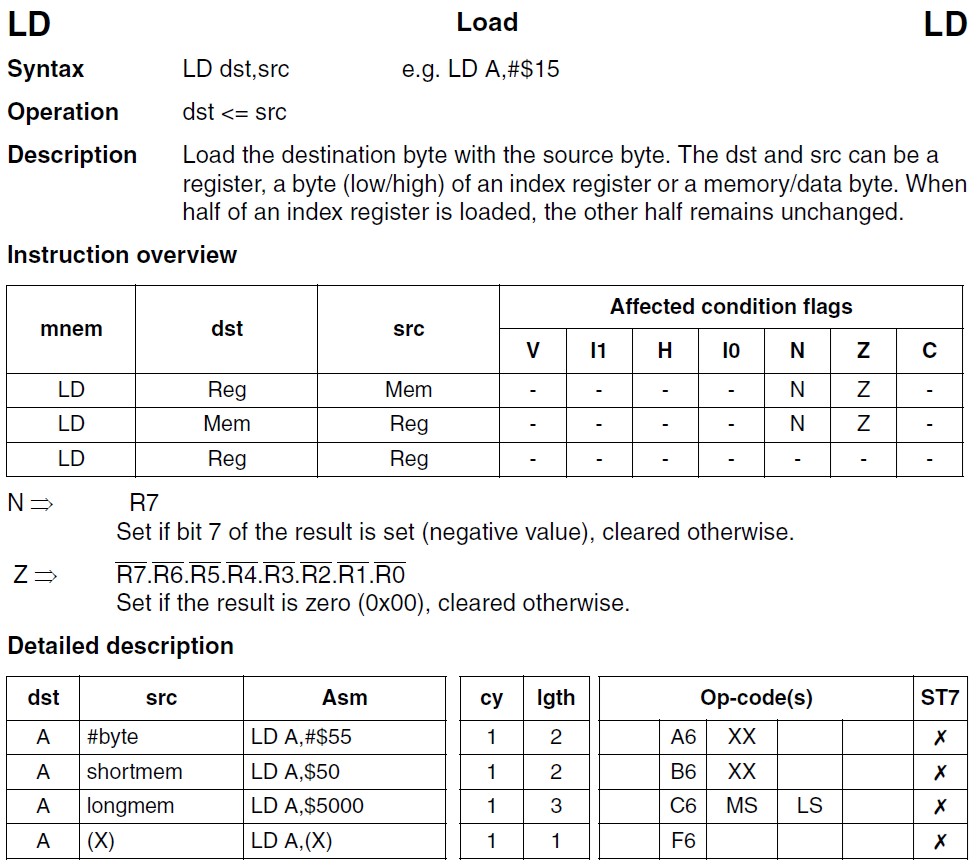
\includegraphics[width=0.7\textwidth]{fig/instr_ld.png}
		\end{center}

	\end{frame}
	
% =====================================================================================================================
	\begin{frame}
    \frametitle{Ukázka režimů adresování STM8S208RB}
		Základní způsoby adresace:
		
		\begin{center}
			\begin{tabular}{l l}
				\textbf{bezprostřední} & \textcolor{blue}{LD A, \#\$hh} \\
				\textbf{přímé} & \textcolor{blue}{LD A, \$hh} \\
				               & \textcolor{blue}{LD A, \$HHhh} \\
				\textbf{indexové} & \textcolor{blue}{LD A, (X)} \\
				                  & \textcolor{blue}{LD A, (\$hh,X)} \\
			\end{tabular}
			\begin{tabular}{| p{5mm} | p{5mm} | p{5mm} | p{5mm} | p{5mm} |}
			\hline
				& A6 & hh &  &  \\
			\hline
				& B6 & hh &  &  \\
			\hline
				& B6 & HH & hh &  \\
			\hline
			  & F6 & & &  \\
			\hline
			  & E6 & hh & &  \\
			\hline
			\end{tabular}
		\end{center}
		
		Pro složitější adresování přibývá prefix:
		
		\begin{center}
			\begin{tabular}{l l}
				\textbf{nepřímé} & \textcolor{blue}{LD A, [\$hh]} \\
				\textbf{nepřímé indexové} & \textcolor{blue}{LD A, ([\$hh],X)} \\
			\end{tabular}
			\begin{tabular}{| p{5mm} | p{5mm} | p{5mm} | p{5mm} | p{5mm} |}
			\hline
				92 & C6 & hh &  &  \\
			\hline
				92 & D6 & hh &  &  \\
			\hline
			\end{tabular}
		\end{center}

	\end{frame}
	
% =====================================================================================================================
	\begin{frame}
    \frametitle{Provádění instrukce STM8S208RB}
		\textbf{Pipeline CPU} - postup vykonání instrukce v několika krocích:
		\small
		
		\begin{minipage}[t][0.35\textheight][t]{0.75\textwidth}
			\begin{enumerate}
				\item \textcolor{blue}{\textbf{FETCH}} - dojde k načtení instrukce z paměti programu,
				\item \textcolor{blue}{\textbf{DECODE}} - dekódování instrukce,
				\item \textcolor{blue}{\textbf{EXECUTE}} - provedení instrukce: operace ALU, operace s pamětí atd.
			\end{enumerate}
		\end{minipage}
		\begin{minipage}[t][0.35\textheight][t]{0.2\textwidth}
		\tiny
		\vspace{0.5mm}
			\begin{center}
				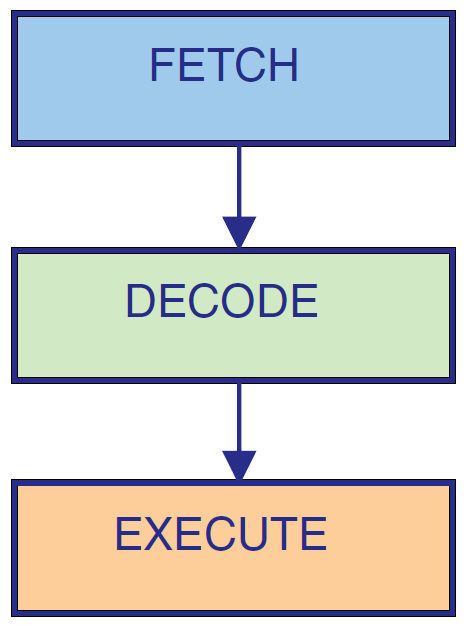
\includegraphics[width=0.90\textwidth]{fig/pipeline.png}
			\end{center}
		\end{minipage}
		
		Lze provádět paralelně:
		
		\begin{center}
			\begin{tabular}{c c c c}
			\textbf{cykl} & \textbf{FETCH} & \textbf{DECODE} & \textbf{EXECUTE} \\ \hline
			1 & instrukce 0 & - & - \\
			2 & instrukce 1 & instrukce 0 & - \\
			3 & instrukce 2 & instrukce 1 & instrukce 0 \\
			\end{tabular}
		\end{center}

	Paralelní čtení instrukcí v pipeline narušují instrukce skoků v programu: \textbf{jmp}, \textbf{call}, \textbf{ret} atd.
	\end{frame}